\section{Intensity Interferometry with Imaging Cherenkov Telescope Array}
Recently, Intensity Interferometry (II) has emerged again as an additional tool to resolve stellar objects as it solves some of the key limitations of classical optical interferometry (atmospheric turbulence, length of baseline, and the sensitivity of the optical aperture). It is suitable for the high-resolution study of very massive, hot, and short-lived stars, such as OB-type, Wolf-Rayet, and Pulsating stars in N-body systems. R. Hanbury Brown and Robert Q. Twiss first installed the Narrabri Stellar Intensity Interferometer (NSII) in 1974 to resolve the diameter of bright stars at visible wavelengths \citep{brown1954lxxiv, brown1974intensity}. Nowadays, Imaging Cherenkov Telescope Arrays (ICTAs), which are primarily used for gamma-ray observations, are at the forefront of implementing II during moonlit nights when it does not detect gamma-ray radiation. As a result, detection of intensity correlation and angular size measurements of stars is going on for highly resolved imaging with optical wavelength, particularly using Very Energetic Radiation Imaging Telescope Array Systems (VERITAS), High Energy Stereoscopic Systems (HESS), and Major Atmospheric Gamma Imaging Cherenkov Telescopes (MAGIC) \citep{kieda2022performance, zmija2022optical, abe2024performance}.

\subsection{The signal for II}\label{sec:signal}
In a simple case, an II consists of two light collectors, for example, MAGIC-I and MAGIC-II, which are pointed to a star and measure the intensity $I_1(t)$ and $I_2(t)$ respectively \citep{acciari2020optical, dravins2013optical}. The signals from both detectors are cross-correlated and averaged over time, which results in an equation form
\begin{equation}
	g^{(2)} = \frac{\left\langle I_1(t) \cdot I_2(t + \tau) \right\rangle}{\langle I_1(t) \rangle \cdot \langle I_2(t) \rangle} 
	\label{eqn:HBT}
\end{equation}
where $\tau$ is the time delay between both telescopes. If the light source is chaotic and randomly polarized, we have:
\begin{equation}
	g^{(2)} = 1 + \frac{\Delta f}{\Delta \nu} \abs{V_{12}}^2
	\label{eqn:HBT2}
\end{equation}
here, $\Delta f$ is the electronic bandwidth, $\Delta \nu$ is the optical bandwidth, and $\Delta f \ll \Delta \nu$ \citep{acciari2020optical}. $V_{12}$ is the Fourier transform of the source brightness distribution and is called complex visibility. Eqn.~\ref{eqn:HBT2} carry the information about the source's structure and shape. However, it loses the phase information due to the presence of only the absolute value of $V_{12}$. In observational astronomy, the correlation in intensity is often expressed in terms of the normalized contrast, given by :
\begin{equation}
	c = \frac{\left\langle \left( I_1(t) - \left\langle I_1 \right\rangle \right) \cdot \left( I_2(t + \tau) - \left\langle I_2 \right\rangle \right) \right\rangle}{\langle I_1(t) \rangle \cdot \langle I_2(t) \rangle} = g^{(2)} - 1
\end{equation}
where, $\left\langle I_1 \right\rangle$ and $\left\langle I_2 \right\rangle$ are the mean intensity from two telescopes.

\subsection{Signal-to-Noise Ratio for Intensity Interferometry}
\begin{figure}
	\centering
	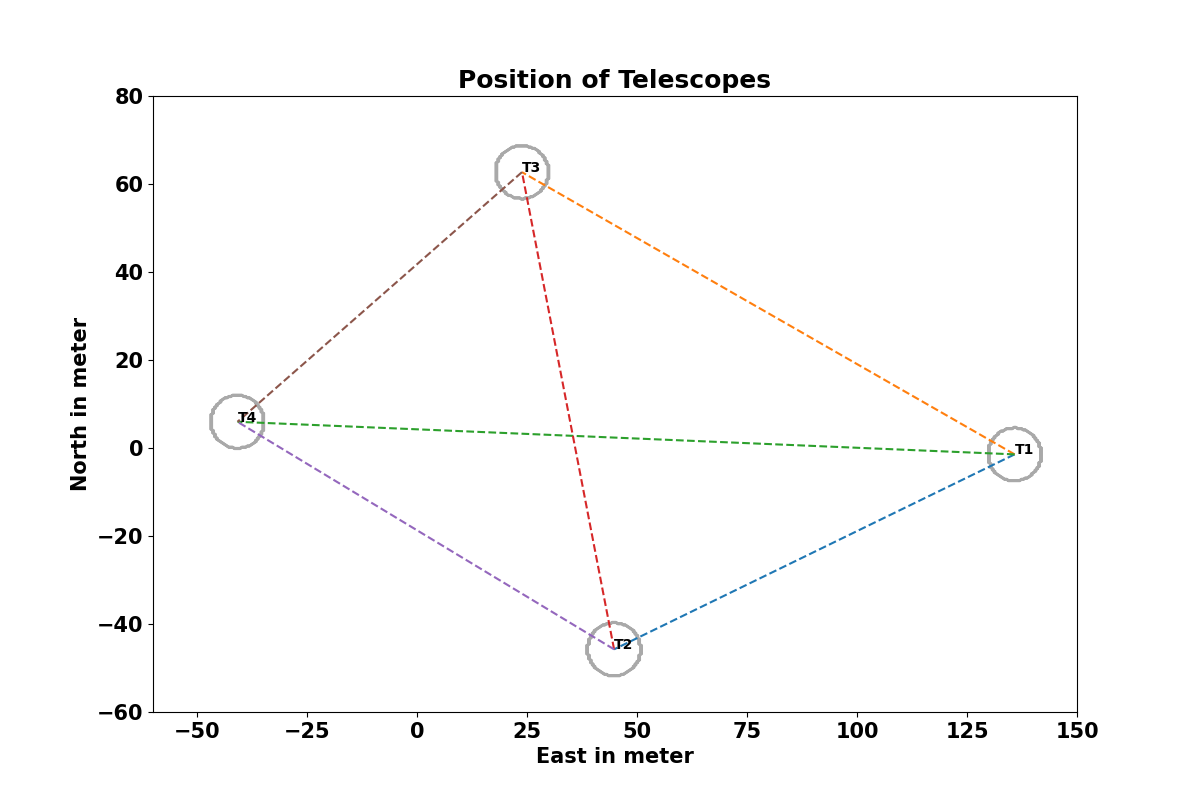
\includegraphics[width=\linewidth]{fig/telescope.png}
	\caption{Configuration of the four Imaging Cherenkov Telescope Array (ICTAs) with similar properties each used to simulate the signal for II.}
	\label{fig:teles}
\end{figure}
The main physics channel of ICTAs is the study of Very High Energy gamma rays ($\geq 30$ GeV) originating from particle showers in the atmosphere. Telescopes have an array of mirrors, which focus the light onto an array of photo-multiplier tubes (PMTs) \citep{aleksic2016major}. Here, Fig.~\ref{fig:teles} shows an arrangement of four ICTAs with similar properties each. For the simulation of II, the light of a stellar source is focused on a single PMT, which has a filter in front. The purpose of this filter is to efficiently transmit light around mean observational frequency, which protects the PMTs from excessive light. It is necessary, as II observations are mainly done during full moon nights when it is too bright for Very High Energy $\gamma$-ray observations. The optical signal of the PMTs is transmitted with optical fibers, converted to an electrical signal, and digitized \citep{acciari2020optical}. The measurable observable is the Pearson's correlation coefficient:
\begin{equation}
	\rho(\tau) = \frac{\left\langle \left( I_1(t) - \left\langle I_1 \right\rangle \right) \cdot \left( I_2(t + \tau) - \left\langle I_2 \right\rangle \right) \right\rangle}{\sqrt{\langle \left( I_1(t) - \langle I_1 \rangle \right)^2 \rangle} \cdot \sqrt{\langle \left( I_2(t) - \langle I_2 \rangle \right) ^2 \rangle}}
	\label{eqn:pearson}
\end{equation}
It must be noted that the calculation of Pearson's correlation coefficient is non-trivial: MAGIC makes use of the convolution theorem for discrete Fourier transforms because it is computationally more efficient. Since $I_1$ and $I_2$ are proportional to the direct current of the PMTs ($DC_i$), the normalized contrast can be calculated as 
\begin{equation}
	c \propto \frac{\rho}{\sqrt{\left(DC_1 \cdot DC_2 \right)}}.
	\label{eq:norm_contrast2}
\end{equation}
One must also correct for a non-constant gain of the PMTs, as well as the moon. The latter can be done by measuring the background light with an additional PMT with no mirrors focused on it \citep{acciari2020optical}.

The significance of the signal is expressed as the signal-to-noise ratio (SNR), which depends on many factors. However, most importantly, SNR is proportional to the absolute value of visibility, which itself depends on the distance between the telescopes \citep{acciari2020optical} 
\begin{equation}
	SNR = A \cdot \alpha \cdot q \cdot n \cdot \abs{V_{12}}^{2}(d) \cdot \sqrt{b_v} \cdot F^{-1} \cdot \sqrt{\frac{T}{2}} \cdot \sigma.
	\label{eq:SNR}
\end{equation}
Here, $A$ is the total mirror area, $\alpha$ the quantum efficiency of the PMTs, $q$ the quantum efficiency of the optics, $n$ the differential photon flux from the source, and $b_v$ the cross-correlation bandwidth. The noise of the PMTs is accounted with $F$, $T$ denotes the observation time, and $\sigma$ is the normalized spectral distribution of the light (including filters) \citep{acciari2020optical}. While most of the parameters can be optimized with hardware, the only way to obtain a better SNR is to increase the observation time with a fixed number of telescopes.  
\begin{figure}
	\centering
	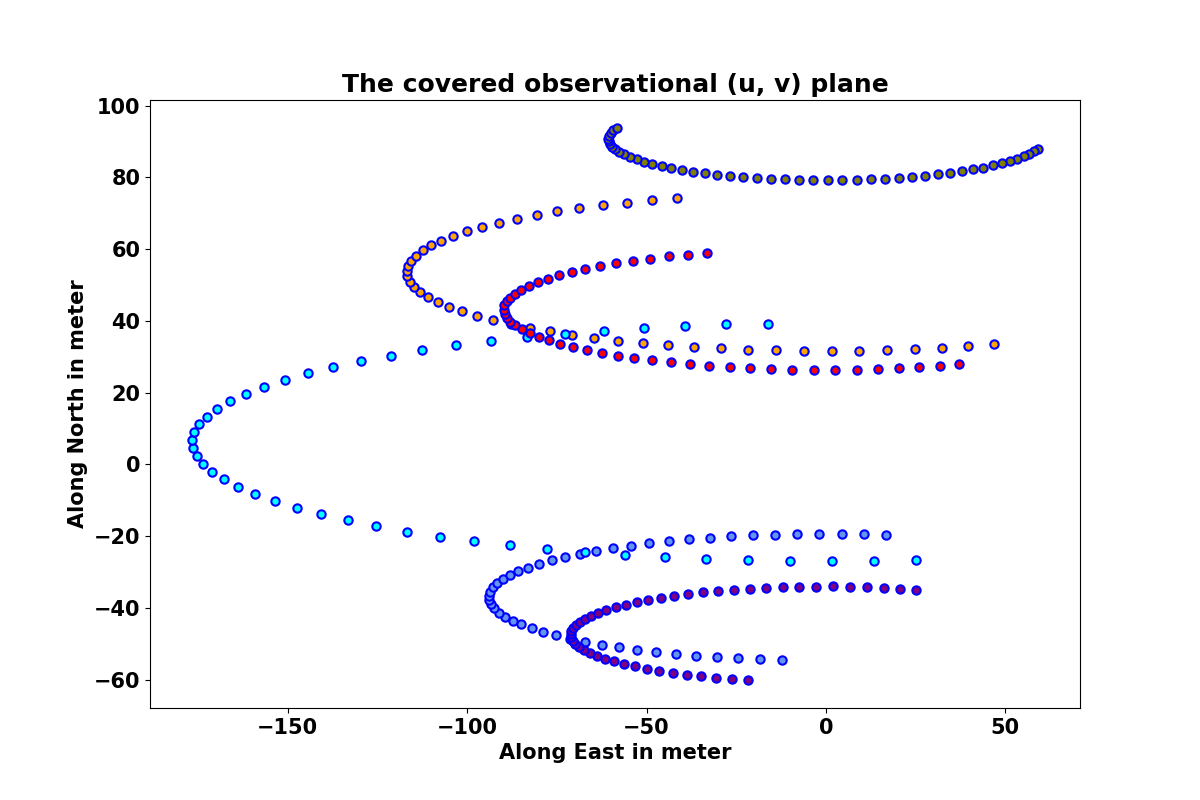
\includegraphics[width=\linewidth]{fig/baseline.png}
	\caption{The tracking of baselines with four telescopes arranged in fig.~\ref{fig:teles} for one night of observation.}
	\label{fig:base}
\end{figure}
\begin{figure}
	\centering
	
\includegraphics[width=0.8\linewidth]{fig/ellipse/ellipse6018.jpg}
	\caption{This figure shows one of the simulated fast-rotating stars. The brightness is highest at the pole and lowest at the equator due to the presence of high-speed rotation of the star. This effect is named gravitational darkening in astronomy.}
	\label{fig:image}
\end{figure}
\subsection{Baseline considerations}
The measurement of the size of stellar objects through absolute visibility depends on the distance between the telescopes, which is called the baseline $B$
\begin{equation}
	V_{12}(B) = \frac{c(B)}{c(0)}.
	\label{eq:angular_size_meas}
\end{equation}
However, this work needs a good SNR value for high precision of measurement, so the large covered observational plane with telescopes is a necessity for II \citep{acciari2020optical, abeysekara2020demonstration}. If the source is at the zenith, the coordinates in the Fourier plane ($u,v$) are given by:
\begin{equation}
	(u,v) = \frac{1}{\lambda} (B_N, B_E)
\end{equation}
where $B_N$ and $B_E$ are the baselines expressed in north and east coordinates. Since not all sources are at the zenith, and the telescopes are stationary, Earth's rotation plays an important role in covering the maximum observational plane through the rotated baselines, which is given as  
\begin{equation}
	\begin{pmatrix} u\\ v\\ w\\ \end{pmatrix} = R_x(\delta) \cdot R_y(h) \cdot R_x(-l) \begin{pmatrix} B_N\\ B_E\\ B_A\\ \end{pmatrix}
	\label{eq:baseline_rot}
\end{equation}
It traces an ellipse for every pair of telescopes. Furthermore, the different altitudes of the telescopes $B_A$ must be considered \citep{dravins2013optical, saha2020theory}. Here, $\delta$ is the declination, and $h$ is the hour angle of the stellar source, and $l$ is the latitude of the telescopes. The three matrices $R_i$ correspond to the fundamental representation of the SO(3) group \citep{saha2020theory}. Fig.~\ref{fig:base} shows the track of six baselines generated from the telescopes (fig.~\ref{fig:teles}) due to Earth's rotation. Since every pair of telescopes traces an ellipse in the Fourier plane, the total number of ellipses scales as follows:
\begin{equation}
	\label{eq:N_telescopes}
	\mathcal{N} = \frac{N_T \cdot (N_T -1)}{2}
\end{equation}

As the number of baselines increases non-linearly, II benefits greatly from a large number of telescopes. The existing and upcoming Cherenkov Telescope Array Observatory (CTAO) can promise to cover the maximum observational plane and provide insight into stellar objects with optical wavelengths in the future.
\begin{figure}
	\centering
	\begin{subfigure}{\linewidth}
		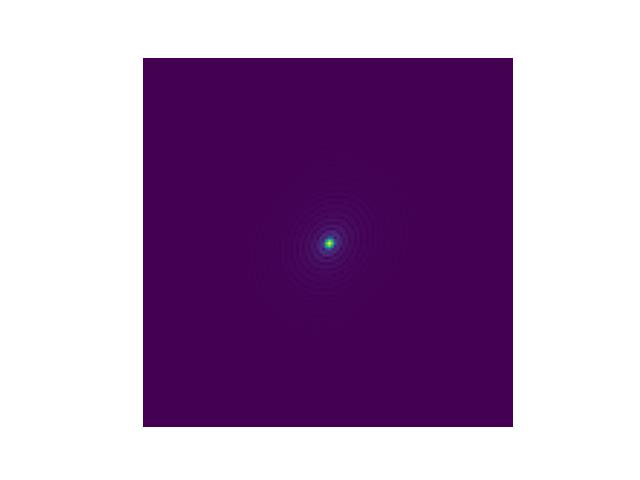
\includegraphics[width=\linewidth]{fig/ft/ft.jpg}
		\caption{The Fourier transform of the source.}
	\end{subfigure}\hfill
	\begin{subfigure}{\linewidth}
		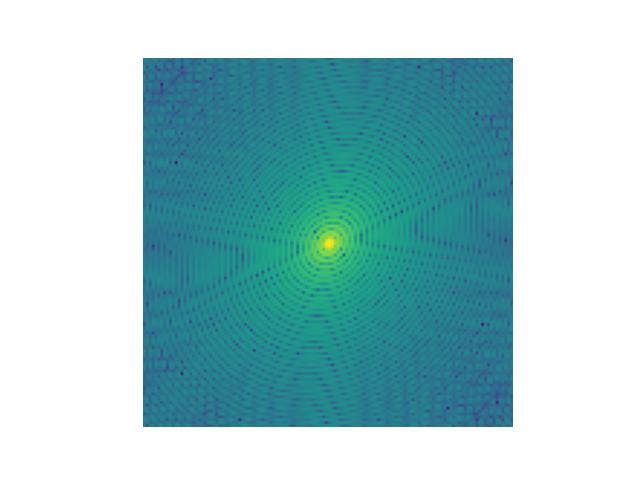
\includegraphics[width=\linewidth]{fig/ft/ft_log.jpg}
		\caption{The logarithmic Fourier transform of the source.}
	\end{subfigure}
	\caption{Absolute value of the two-dimensional Fast Fourier Transform of Fig.~\ref{fig:image} on linear and logarithmic scales. Observation of the maximum (u, v) plane with a finite number of baselines can be completed with the help of Earth's rotation.}
	\label{fig:ft}
\end{figure}
\begin{figure}
	\centering
	\begin{subfigure}{\linewidth}
		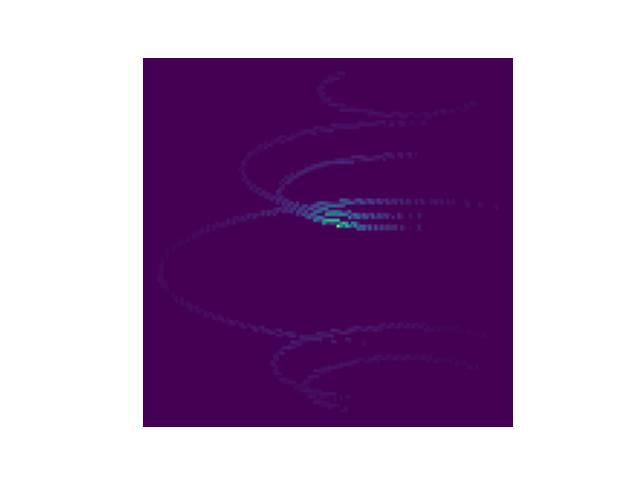
\includegraphics[width=\linewidth]{fig/ft/ft_base.jpg}
		\caption{The Fourier transform with baselines.}
	\end{subfigure}\hfill
	\begin{subfigure}{\linewidth}
		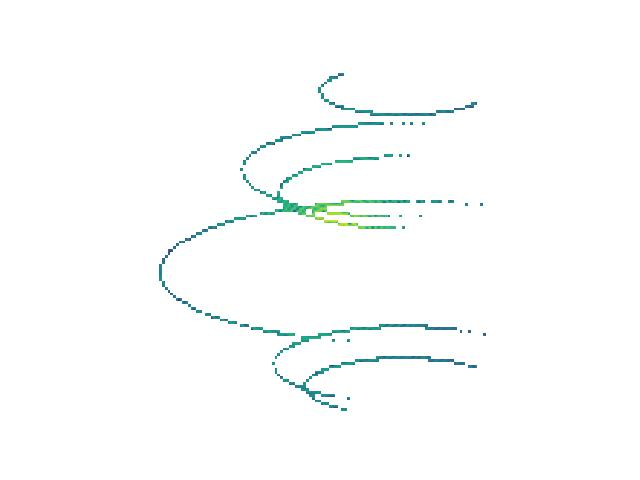
\includegraphics[width=\linewidth]{fig/ft/ft_log_base.jpg}
		\caption{The logarithmic Fourier transform with baselines.}
	\end{subfigure}
	\caption{The upper panel shows the absolute value of the two-dimensional Fast Fourier Transform of Fig.~\ref{fig:image} measured by baselines shown in Fig.~\ref{fig:teles} on a linear scale, and the lower panel shows the same on a logarithmic scale.}
	\label{fig:ft_base}
\end{figure}
\subsection{An Object: Fast Rotating Stars}
In our work, we simulate a single fast-rotating star to test image reconstruction with II in intersection with the Generative Adversarial Networks (GAN). Fast rotation causes stars to take on an oblate shape, flattening at the poles and bulging at the equator due to the existence of stronger centrifugal force \citep{von1924radiative, 1999A&A...347..185M}. Fig.~\ref{fig:image} shows one of the simulations of a fast-rotating star, where the star takes on an elliptical shape with brightness distributed across the object. The brightness is maximum at the poles and minimum at the equator, a phenomenon known as gravity darkening \citep{lucy1967gravity}. This effect was first observed in the fast-rotating star Regulus through interferometric and spectroscopic data from the Center for High Angular Resolution Astronomy (CHARA) Array \citep{mcalister2005first}. These stars are crucial for understanding a variety of astrophysical processes and help to understand the stellar evolution, internal structure, and rotational dynamics over time.

Intensity Interferometry (II) detects the photon from the stellar objects, and the correlation of it results in squared visibility (explained in subsection.\ref{sec:signal}). According to Van Cittert Zernike's theorem, this signal is the Fourier transform of brightness distribution in the sky. Fig.~\ref {fig:ft} visualize this statement for the source shown in Fig.~\ref{fig:image} using II on linear and logarithmic scales. However, current observational techniques are unable to capture the full signal, and only partial data can be collected with a single night's simulation, which has been shown in Fig.~\ref{fig:ft_base}. It is the covered observational plane using the baselines shown in Fig.~\ref{fig:teles} on linear and logarithmic scales, respectively. However, the instrumentation of existing and upcoming CTAO shows the possibility of covering the maximum observable portion of the visibility plane for stellar objects, offering high resolution to understand the stellar structure and its evolution with time.